%!LW recipe=pdfLaTeXmk
\documentclass[scheme=plain,aspectratio=169]{beamer}
\usepackage[T1]{fontenc}
\usepackage{fontawesome5}
\usepackage{mathtools}
\usepackage{tikz}
\usepackage{booktabs}
\usepackage{caption}
\usepackage{outlines}
\usepackage{graphicx}
\usepackage{tabularray}
\usepackage{hyperref}
\usepackage{url}
\usepackage{xspace}
\usepackage{qrcode}
\usepackage{soul}
\usepackage{tgheros}
\usepackage[style=numeric, backend=biber, url=false, doi=false, isbn=false]{biblatex}
\addbibresource{custom.bib}
\addbibresource{iclr2026_conference.bib}
\addbibresource{talk.bib}
\renewcommand{\cite}{\footfullcite}

\usetheme[
    progressbar=frametitle,
    numbering=fraction,
    subsectionpage=progressbar,
    titleformat title=smallcaps,
    titleformat subtitle=smallcaps,
    titleformat section=smallcaps,
    titleformat frame=smallcaps]{moloch}

\setbeamercolor{palette primary}{bg=gray1}
\setbeamercolor{frametitle}{bg=black,fg=white}
\setbeamercolor{progress bar}{fg=black}
\setbeamerfont{footnote}{size=\tiny}

\definecolor{barpos}{HTML}{2F6E73}
\definecolor{barneg}{HTML}{C0392B}
\definecolor{tickgray}{HTML}{9A9A9A}
\definecolor{barbase}{HTML}{9A9A9A}
\definecolor{barsft}{HTML}{93C0C4}
\definecolor{ctxbg}{HTML}{F9D5BC}
\definecolor{ctxfg}{HTML}{B5551F}
\definecolor{rsnbg}{HTML}{EAF3B5}
\definecolor{rsnfg}{HTML}{6B7A12}
\definecolor{actbg}{HTML}{C3DBF3}
\definecolor{actfg}{HTML}{2F5597}

\usetikzlibrary{calc,arrows.meta,decorations.pathreplacing,positioning}
\setcounter{tocdepth}{1}

\makeatletter
\newlength{\frametitle@padding}
\setlength{\frametitle@padding}{2.2ex}
\newcommand{\frametitlestrut@start}{
  \rule{0pt}{\frametitle@padding +%
    \totalheightof{%
      \ifcsdef{frametitleformat}{\frametitleformat X}{X}%
    }%
  }%
}
\newcommand{\frametitlestrut@end}{
  \rule[-\frametitle@padding]{0pt}{\frametitle@padding}
}
\setbeamertemplate{frametitle}{
    \nointerlineskip%
    \begin{beamercolorbox}[%
        wd=\paperwidth,%
        sep=0pt,%
        leftskip=\frametitle@padding,%
        rightskip=\frametitle@padding,%
      ]{frametitle}%
    \frametitlestrut@start%
    \insertframetitle%
    \hfill%
    \nolinebreak%
    \frametitlestrut@end%
    \end{beamercolorbox}%
    \begin{tikzpicture}[remember picture,overlay]
        \coordinate (logo) at ([xshift=-1.8cm,yshift=-0.5cm]current page.north east);
        \node at (logo) {
\includegraphics[height=.1\textheight]{figures/northeastern.eps}};
    \end{tikzpicture}
}
\makeatother

\setbeamertemplate{footline}{
    \hbox{
    \begin{beamercolorbox}[wd=\paperwidth,ht=3ex,dp=1.5ex,leftskip=2ex,rightskip=2ex]{page footer}%
        \usebeamerfont{title in head/foot}%
        \hfill
        \begin{tblr}{
            width=.8\linewidth,
            colspec={X[5,l]X[r]}
        }
            \insertsectionhead{}
            &
            \insertframenumber{} / \inserttotalframenumber
        \end{tblr}
        \hfill{}
    \end{beamercolorbox}}%
}

\defbeamertemplate{section page}{my progressbar}{
  \centering
  \begin{beamercolorbox}[wd=\paperwidth,leftskip=10mm,rightskip=10mm,sep=0pt]{section page}
    \begin{minipage}{0.9\linewidth}
      \raggedright
      \usebeamercolor[fg]{section title}
      \usebeamerfont{section title}
      \insertsection\\[-0.5\baselineskip]
      \usebeamertemplate*{progress bar in section page}
      \par
    \end{minipage}
  \end{beamercolorbox}
  \par
}
\setbeamertemplate{section page}[my progressbar]

\UseTblrLibrary{booktabs}
\graphicspath{ {./figures/} }

\DeclareRobustCommand{\projectname}{\textsc{Firefly}\xspace}

% \figorplaceholder[height]{path}{planned figure}: image if the file exists, else a dashed placeholder box
\newcommand{\figorplaceholder}[3][.78\textheight]{%
  \IfFileExists{#2}{\includegraphics[height=#1]{#2}}{%
    \begin{tikzpicture}
      \node[draw=gray, dashed, rounded corners, minimum width=.9\linewidth, minimum height=#1,
            text width=.8\linewidth, align=left, font=\footnotesize, text=gray]
        {\textbf{[Figure placeholder]} \texttt{#2}\\[4pt] #3};
    \end{tikzpicture}}}

% the "pick two" triangle; #1 = what goes in the centre
\newcommand{\picktwotriangle}[1]{%
  \begin{tikzpicture}[
      vert/.style={circle, fill=barpos, text=white, font=\small\bfseries, minimum size=1.9cm, inner sep=2pt, align=center},
      edge/.style={line width=2.5pt, barbase!55},
      elab/.style={fill=white, inner sep=4pt, font=\small, align=center}]
    \coordinate (S) at (90:3.1);
    \coordinate (R) at (210:3.1);
    \coordinate (V) at (330:3.1);
    \draw[edge] (S) -- (R);
    \draw[edge] (R) -- (V);
    \draw[edge] (V) -- (S);
    \node[vert] at (S) {Scalable};
    \node[vert] at (R) {Real};
    \node[vert] at (V) {Verifiable};
    \node[elab] at ($(S)!0.5!(R)$) {Task-first\\synthesis\\{\color{barneg}\faTimes~not verifiable}};
    \node[elab] at ($(R)!0.5!(V)$) {Human\\annotation\\{\color{barneg}\faTimes~not scalable}};
    \node[elab] at ($(V)!0.5!(S)$) {Simulated\\APIs\\{\color{barneg}\faTimes~not real}};
    #1
  \end{tikzpicture}}

\title{\projectname: Illuminating Large-Scale Verified Tool-Call Data Generation from Real APIs}
% TODO: affiliations for the non-Northeastern co-authors
\author{{\small \textbf{Yuxuan Lu}, Ziyi Wang, Yingzhou Lu, Yisi Sang, Jiri Gesi,\\ Xianfeng Tang, Yimeng Zhang, Zhenwei Dai, Hui Liu, Hanqing Lu,\\ Chen Luo, Qi He, Benoit Dumoulin, Jing Huang, Dakuo Wang}}
\institute{Northeastern University \quad | \quad \url{https://yuxuan.lu}}
\date{Oct 2026}
\titlegraphic{
\includegraphics[height=1.6cm]{figures/neurips-logo.pdf}}

\begin{document}

\maketitle

\begin{frame}{Agents Call Tools: WebGPT (2021)}
  \centering
  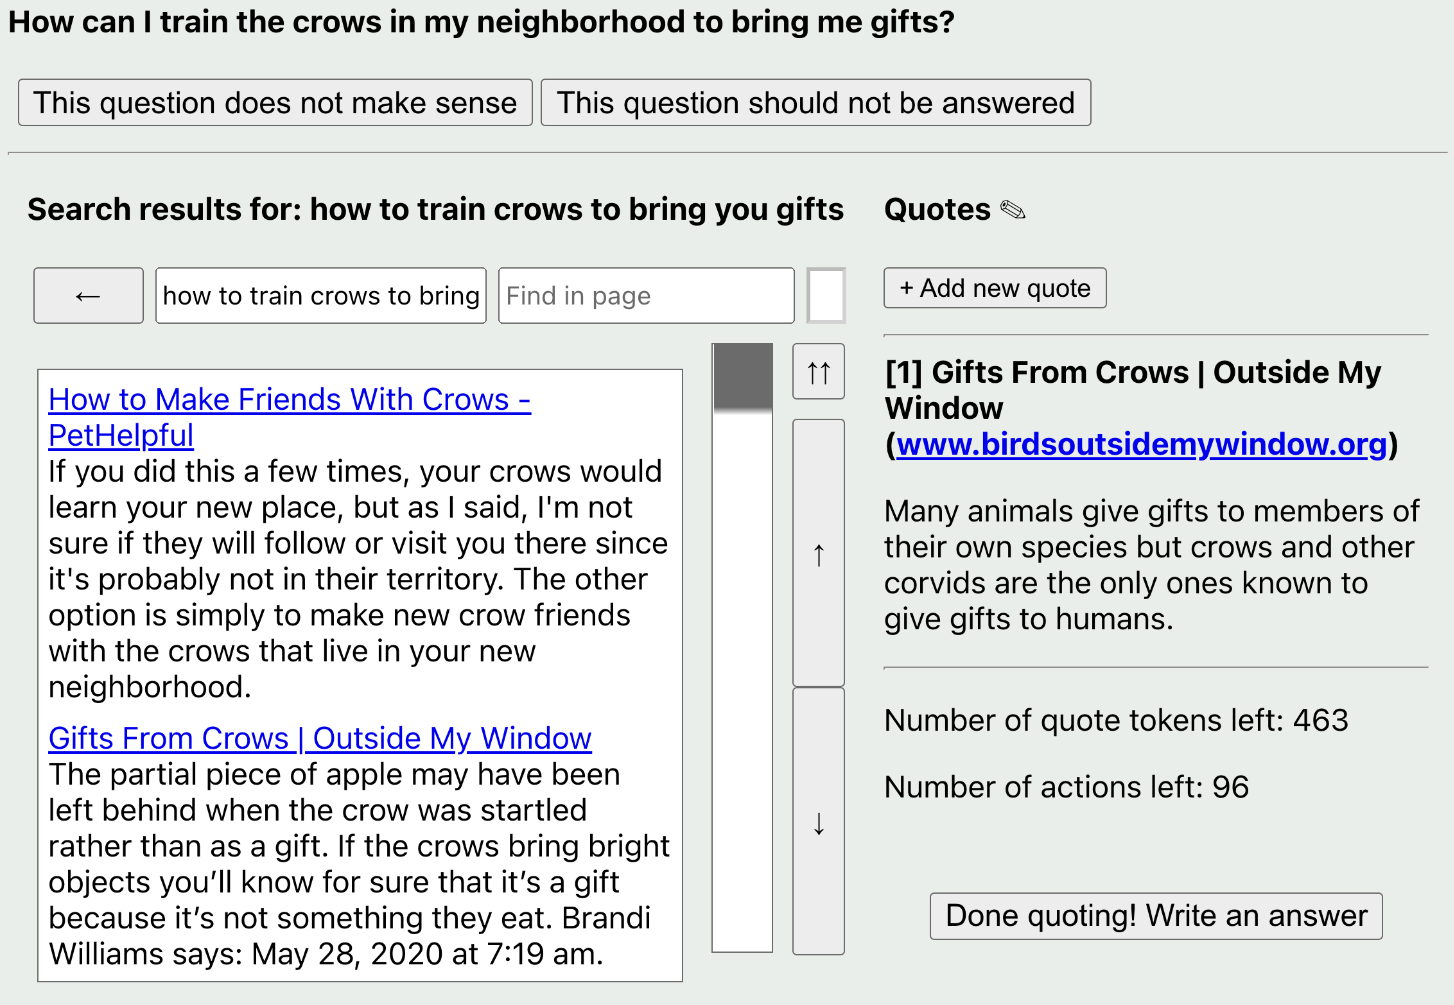
\includegraphics[height=.68\textheight]{figures/webgpt.png}\\[6pt]
  {\small The browser is the tool: the model calls \texttt{search}, \texttt{click}, \texttt{quote}.}
\end{frame}

{
\setbeamercolor{background canvas}{bg=white}
\begin{frame}[plain]
  \centering
  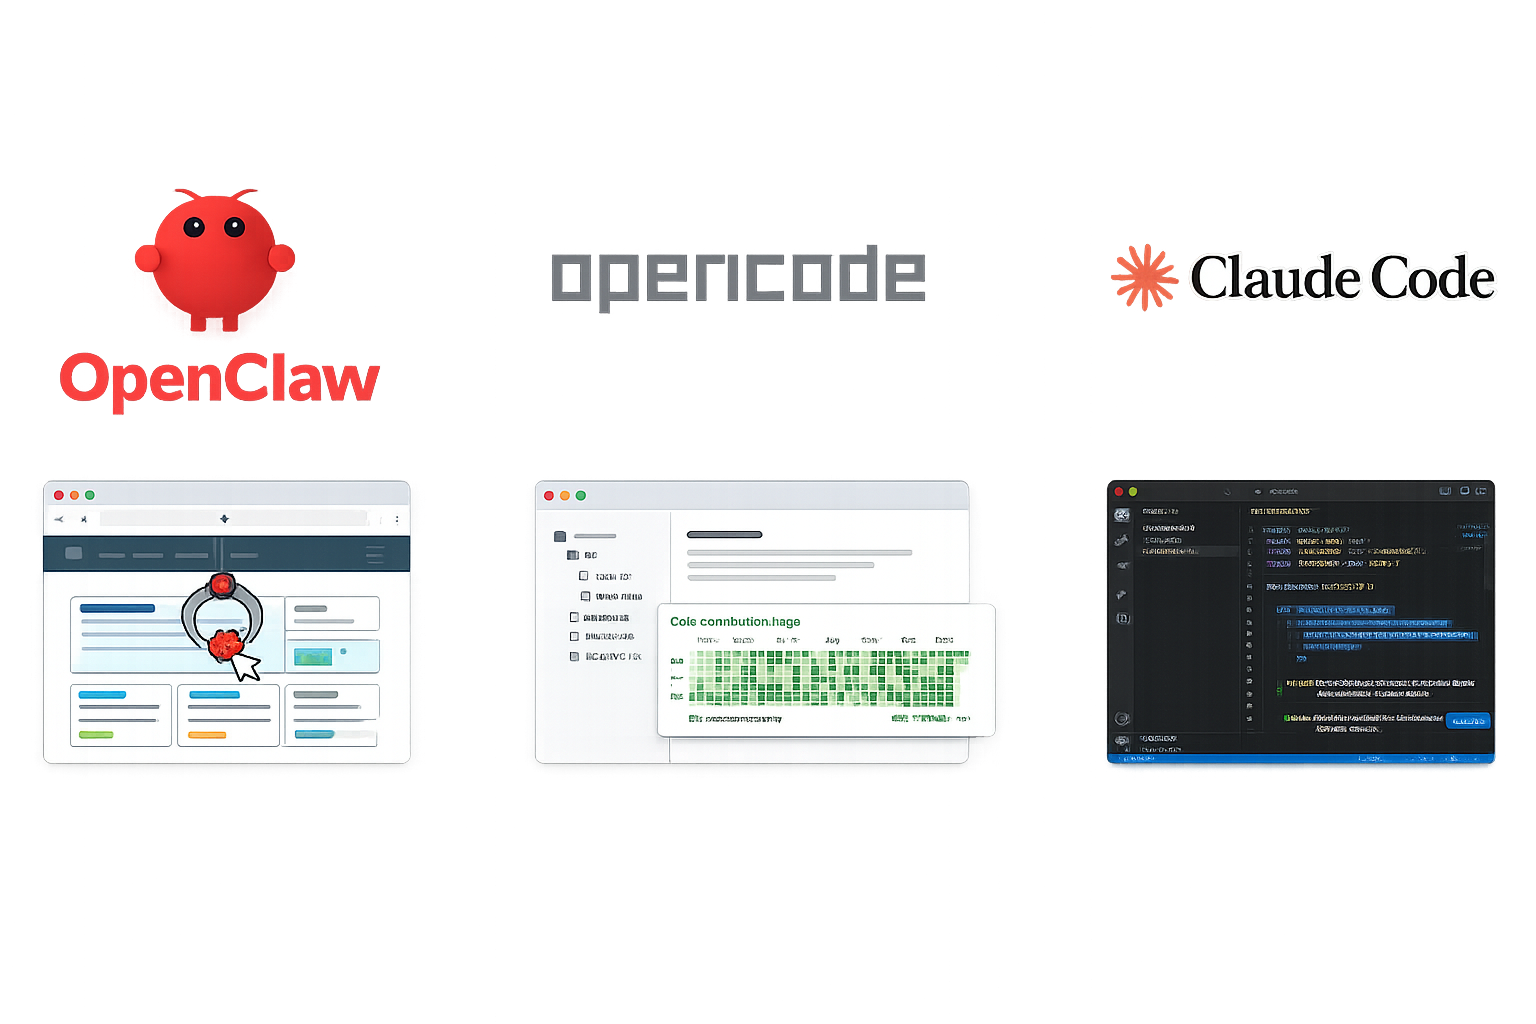
\includegraphics[width=.8\linewidth]{figures/agents.png}
\end{frame}
}

{
\setbeamercolor{background canvas}{bg=black}
\begin{frame}[plain]
  \begin{tikzpicture}[remember picture,overlay]
    \node[anchor=center, inner sep=0] at (current page.center) {
      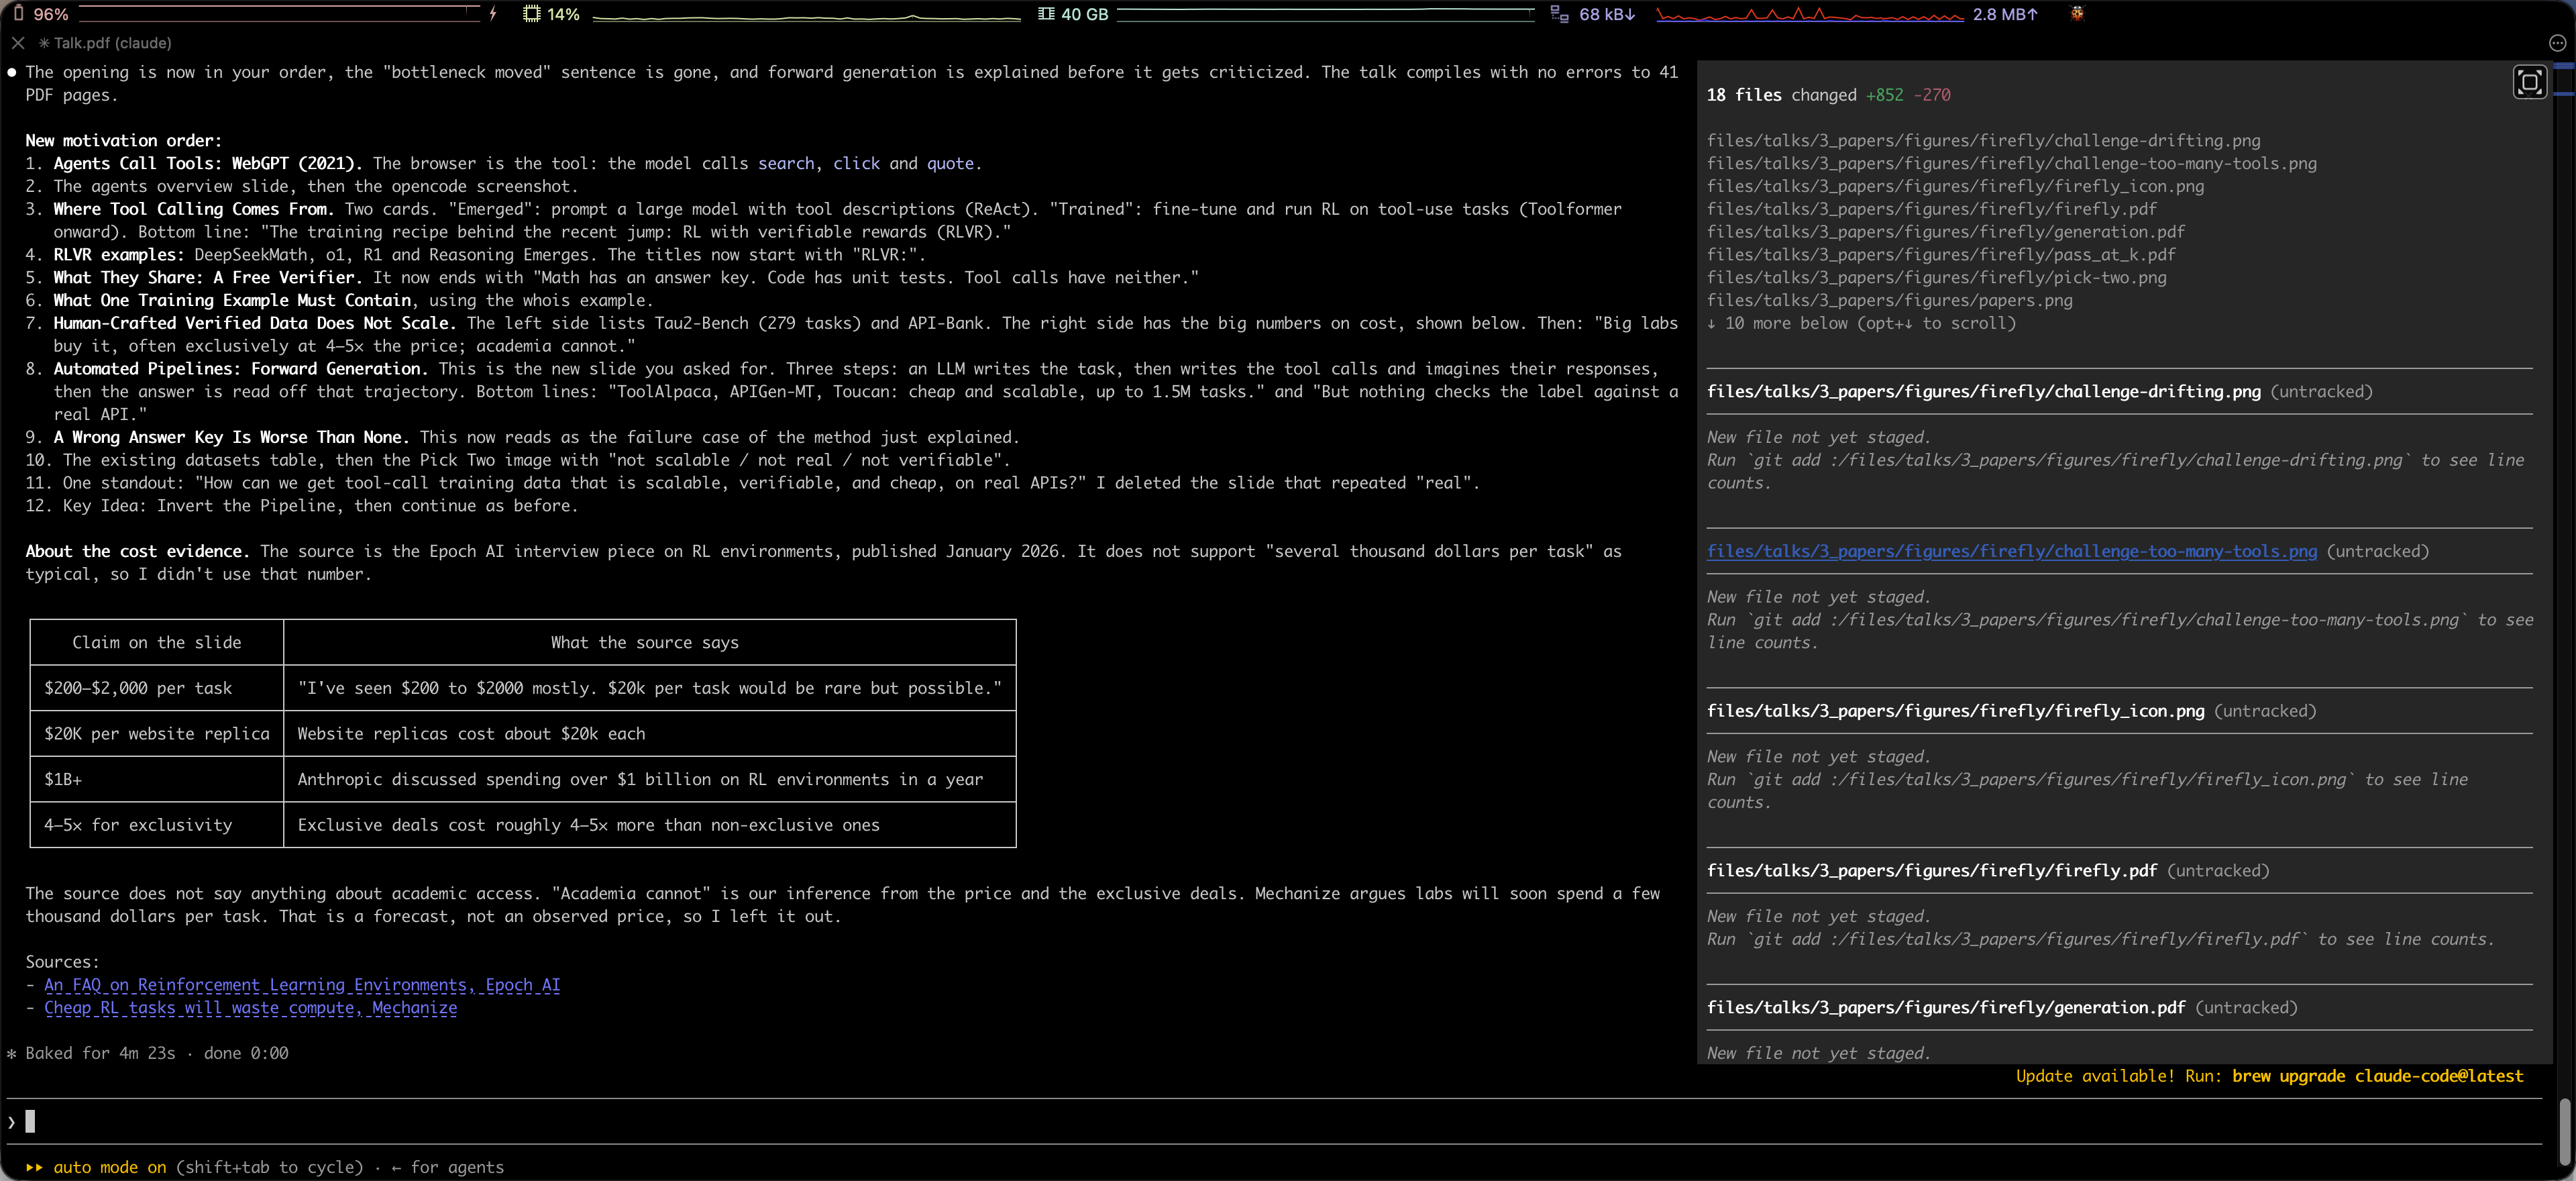
\includegraphics[width=\paperwidth, height=\paperheight, keepaspectratio]{figures/claude-code-screenshot.png}
    };
  \end{tikzpicture}
\end{frame}
}

\begin{frame}{Where Tool Calling Comes From}
  \centering
  \resizebox{.96\linewidth}{!}{%
  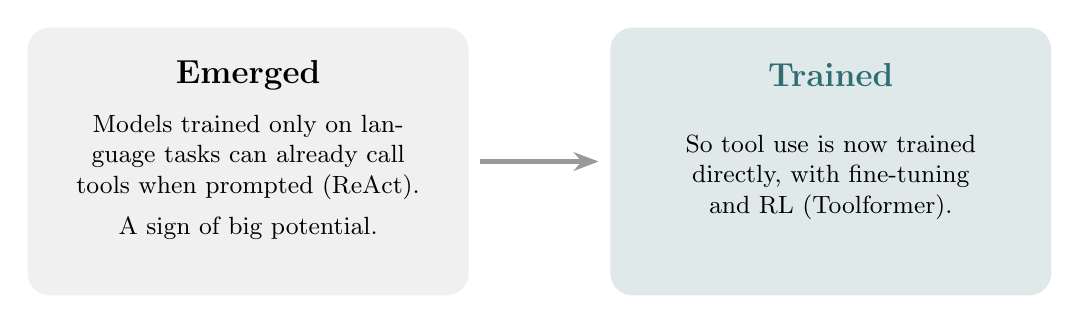
\begin{tikzpicture}[
      card/.style={rounded corners=8pt, minimum width=5.6cm, minimum height=3.4cm},
      hd/.style={font=\large\bfseries},
      ds/.style={font=\small, text width=5cm, align=center},
      arr/.style={-{Stealth[length=9pt]}, line width=2pt, tickgray}]
    \node[card, fill=gray!12] at (0,0) {};
    \node[hd] at (0,1.1) {Emerged};
    \node[ds] at (0,-0.2) {Models trained only on language tasks can already call tools when prompted (ReAct).\\[4pt] A sign of big potential.};
    \node[card, fill=barpos!15] at (7.4,0) {};
    \node[hd, barpos] at (7.4,1.1) {Trained};
    \node[ds] at (7.4,-0.2) {So tool use is now trained directly, with fine-tuning and RL (Toolformer).};
    \draw[arr] (2.95,0) -- (4.45,0);
  \end{tikzpicture}}\\[14pt]
  {\small\bfseries The training recipe behind the recent jump: RL with verifiable rewards (RLVR).}
\end{frame}

\begin{frame}{RLVR: DeepSeekMath (2024)}
  \begin{columns}[c]
    \begin{column}{0.58\linewidth}
      \centering
      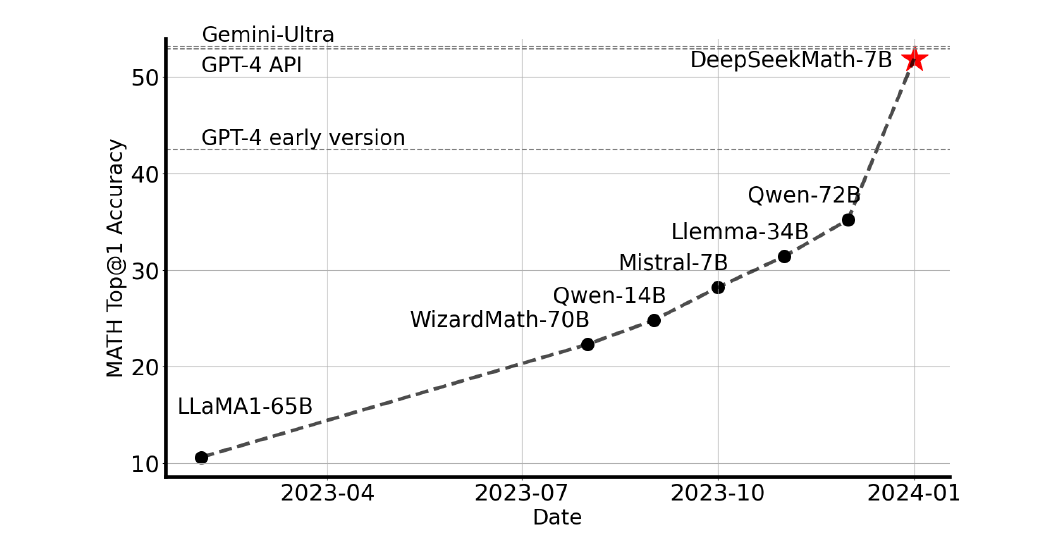
\includegraphics[width=\linewidth]{figures/deepseekmath-math.png}
    \end{column}
    \begin{column}{0.42\linewidth}
      {\color{barpos}\fontsize{40}{44}\selectfont\textbf{51.7\%}}\\[2pt]
      {\small on competition-level MATH with a 7B model, approaching Gemini-Ultra and GPT-4}\\[14pt]
      {\small Introduced \textbf{GRPO}: RL where the reward is simply whether the final answer matches.}
    \end{column}
  \end{columns}
\end{frame}

\begin{frame}{RLVR: OpenAI o1 (2024)}
  \centering
  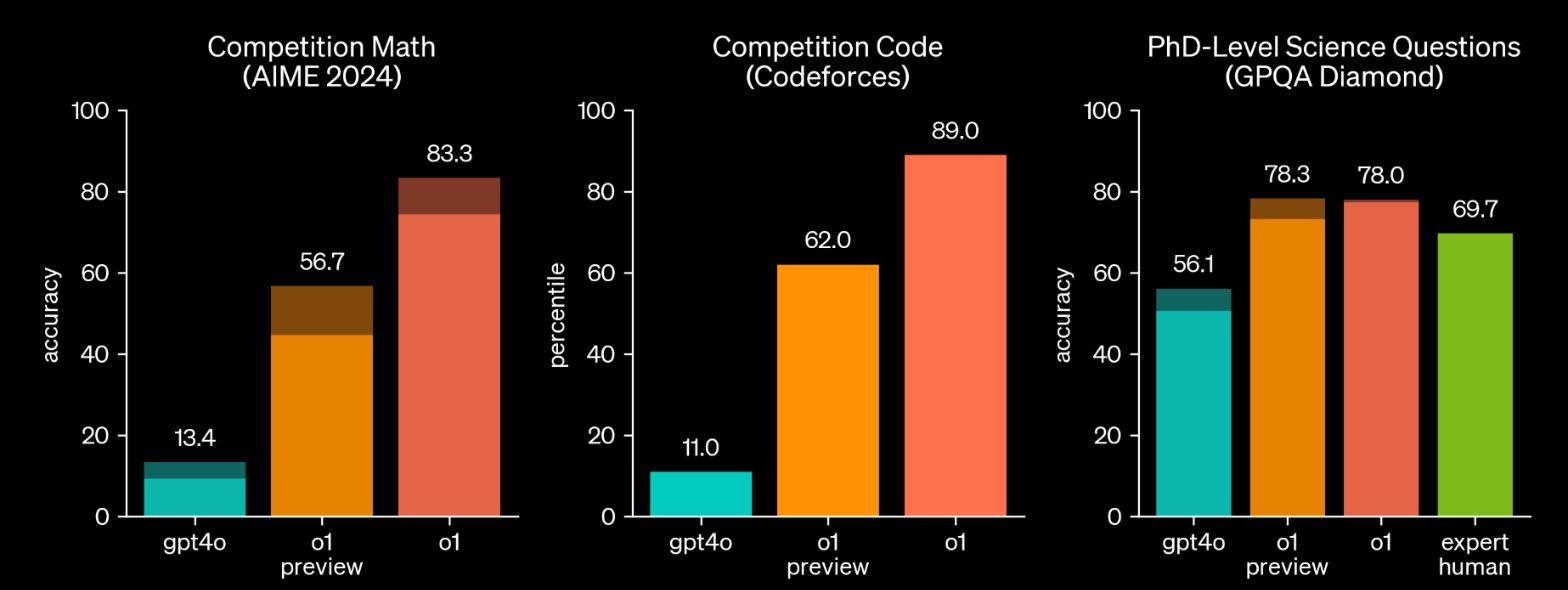
\includegraphics[width=.92\linewidth]{figures/o1-benchmarks.png}\\[10pt]
  {\small Large-scale RL teaches the model to think before it answers.}\\
  {\small\bfseries AIME 13.4 $\rightarrow$ 83.3, Codeforces percentile 11 $\rightarrow$ 89 over GPT-4o.}
\end{frame}

\begin{frame}{What RLVR Needs}
  \centering
  \resizebox{.96\linewidth}{!}{%
  \begin{tikzpicture}[
      box/.style={rounded corners=6pt, inner sep=7pt, align=center, font=\small},
      att/.style={rounded corners=3pt, fill=actbg, text=actfg, font=\ttfamily\scriptsize, minimum width=1.7cm, minimum height=0.5cm},
      hd/.style={font=\small\bfseries},
      arr/.style={-{Stealth[length=6pt]}, line width=1.2pt, tickgray}]
    % task with key
    \node[hd] at (0,1.6) {Task};
    \node[box, fill=rsnbg, text width=3.3cm, execute at begin node={\hyphenpenalty=10000}] (task) at (-0.2,0) {a question\\ \textbf{+ its ground truth /\\ evaluation rubric}};
    % policy
    \node[hd] at (3.4,1.6) {1. Roll out};
    \node[font=\fontsize{26}{26}\selectfont] (bot) at (3.4,0.1) {\faRobot};
    \node[font=\footnotesize, anchor=north] at (bot.south) {policy};
    % attempts
    \node[att] (a1) at (6.2,0.75)  {attempt 1};
    \node[att] (a2) at (6.2,0)     {attempt 2};
    \node[att] (a3) at (6.2,-0.75) {attempt 3};
    % verify
    \node[hd] at (9.2,1.6) {2. Verify};
    \node[barpos, font=\large] (v1) at (9.2,0.75)  {\faCheck};
    \node[barneg, font=\large] (v2) at (9.2,0)     {\faTimes};
    \node[barpos, font=\large] (v3) at (9.2,-0.75) {\faCheck};
    \node[font=\footnotesize, align=center] at (9.2,-1.55) {compare with the ground\\ truth / evaluation rubric};
    % reward
    \node[hd] at (12.0,1.6) {3. Reward};
    \node[box, fill=gray!12, font=\ttfamily\small] (rw) at (12.0,0) {1\\0\\1};
    % arrows
    \draw[arr] (task) -- (bot);
    \draw[arr] (bot.east) -- (a1.west);
    \draw[arr] (bot.east) -- (a2.west);
    \draw[arr] (bot.east) -- (a3.west);
    \draw[arr] (a1) -- (v1);
    \draw[arr] (a2) -- (v2);
    \draw[arr] (a3) -- (v3);
    \draw[arr] (10.0,0) -- (rw.west);
    \draw[arr] (rw.south) |- (7.7,-2.4) -| (3.4,-0.8);
    \node[font=\footnotesize, text=black, fill=white, inner sep=2pt] at (7.7,-2.4) {4. update the policy toward the rewarded attempts};
  \end{tikzpicture}}
\end{frame}

\begin{frame}{RLVR for Tool Calling Needs}
  \centering
  \resizebox{.72\linewidth}{!}{%
  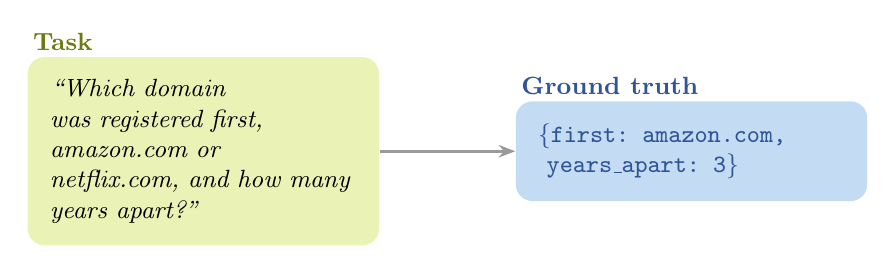
\begin{tikzpicture}[
      box/.style={rounded corners=6pt, inner sep=8pt, align=left, text width=3.9cm,
                  execute at begin node={\hyphenpenalty=10000}},
      hd/.style={font=\small\bfseries, anchor=south west, inner sep=2pt},
      arr/.style={-{Stealth[length=6pt]}, line width=1.2pt, tickgray}]
    \node[box, fill=rsnbg, font=\small\itshape] (t) at (0,0)
      {``Which domain was registered first, amazon.com or netflix.com, and how many years apart?''};
    \node[box, fill=actbg, text=actfg, font=\ttfamily\small] (a) at (6.2,0)
      {\{first: amazon.com,\\ \ years\_apart: 3\}};
    \node[hd, rsnfg] at (t.north west) {Task};
    \node[hd, actfg] at (a.north west) {Ground truth};
    \draw[arr] (t) -- (a);
  \end{tikzpicture}}\\[14pt]
  {\small {\color{barpos}\faCheck}~a natural task \qquad
          {\color{barpos}\faCheck}~an answer that is actually correct}\\[6pt]
  {\small\bfseries For thousands of tasks, across hundreds of APIs.}
\end{frame}

\begin{frame}{Human-Crafted Verified Data Does Not Scale}
  \begin{columns}[c]
    \begin{column}{0.44\linewidth}
      {\small\bfseries Open, human-curated tool-use data}\\[6pt]
      {\small \textbf{Tau2-Bench}: 279 tasks over 68 APIs, each with a hand-checked goal state.}\\[6pt]
      {\small \textbf{API-Bank}: 1,888 annotated tool-use dialogues.}\\[10pt]
      {\small Carefully verified, but small, and built one task at a time.}
    \end{column}
    \begin{column}{0.54\linewidth}
      {\color{barpos}\fontsize{24}{28}\selectfont\textbf{\$200--\$2,000}}\\
      {\small typical price of one RL task bought by AI labs}\\[4pt]
      {\color{barpos}\fontsize{24}{28}\selectfont\textbf{\$20K}}\\
      {\small for one replicated website to train in}\\[4pt]
      {\color{barpos}\fontsize{24}{28}\selectfont\textbf{\$1B+}}\\
      {\small Anthropic discussed spending on RL environments in a year}
    \end{column}
  \end{columns}
  \vspace{10pt}
  \centering {\small Big labs buy it, often exclusively at 4--5$\times$ the price; academia cannot.}\\
  {\small\bfseries Verified, but every new task and API costs more money.}
\end{frame}

\begin{frame}{Automated Pipelines: Forward Generation}
  \centering
  \resizebox{.96\linewidth}{!}{%
  \begin{tikzpicture}[
      box/.style={rounded corners=6pt, inner sep=8pt, align=left, text width=3.9cm, minimum height=3.1cm,
                  execute at begin node={\hyphenpenalty=10000}},
      hd/.style={font=\small\bfseries, anchor=south west, inner sep=2pt},
      arr/.style={-{Stealth[length=6pt]}, line width=1.2pt, tickgray}]
    \node[box, fill=gray!12, font=\small] (t) at (0,0)
      {Input: all tool descriptions.\\[4pt] An LLM writes a task that uses these tools.};
    \node[box, fill=gray!12, font=\small] (tr) at (5.3,0)
      {A separate solver model rolls out a trajectory of tool calls for that task.};
    \node[box, fill=gray!12, font=\small] (a) at (10.6,0)
      {The solver's final answer becomes the ground truth.};
    \node[hd] at (t.north west) {1. Write the task};
    \node[hd] at (tr.north west) {2. Solver rollout};
    \node[hd] at (a.north west) {3. Ground truth};
    \draw[arr] (t) -- (tr);
    \draw[arr] (tr) -- (a);
    \node<2->[font=\small, text=barneg, text width=4.1cm, align=left, anchor=north,
          execute at begin node={\hyphenpenalty=10000}] at (0,-1.85)
      {\faTimes~The task may be impossible: its final state is unreachable.};
    \node<2->[font=\small, text=barneg, text width=4.1cm, align=left, anchor=north,
          execute at begin node={\hyphenpenalty=10000}] at (5.3,-1.85)
      {\faTimes~The solver may get it wrong: then the ground truth is wrong.};
    \path (0,-3.3);
  \end{tikzpicture}}\\[12pt]
  \visible<2->{{\small ToolAlpaca, APIGen-MT, Toucan: scalable, up to 1.5M tasks.}\\[4pt]
  {\small\bfseries Nothing guarantees the ground truth is correct.}}
\end{frame}

\begin{frame}{Scalable, Real, Verifiable: Pick Two}
  \centering
  \figorplaceholder[.66\textheight]{figures/pick-two.png}{Three panels, yellow robot style: Human annotation, Simulated APIs, Task first.}\\[6pt]
  {\small {\color{barneg}\faTimes}~not scalable \qquad
          {\color{barneg}\faTimes}~not real \qquad
          {\color{barneg}\faTimes}~not verifiable}
\end{frame}

\begin{frame}[standout]
  How can we get tool-call training data that is \ul{scalable}, \ul{real}, and \ul{verifiable}?
\end{frame}

\begin{frame}{Key Idea: Invert the Pipeline}
  \centering
  \resizebox{\linewidth}{!}{%
  \begin{tikzpicture}[
      box/.style={rounded corners=5pt, minimum height=1cm, minimum width=2.6cm, font=\small, align=center},
      arr/.style={-{Stealth[length=6pt]}, line width=1.2pt, tickgray},
      lbl/.style={font=\small\bfseries, anchor=east, align=right}]
    \node[lbl] at (-0.3,0) {Forward generation\\{\footnotesize\mdseries prior work}};
    \node[box, fill=gray!15] (t1)  at (1.3,0) {Task\\{\footnotesize written first}};
    \node[box, fill=gray!15] (tr1) at (4.9,0) {Trajectory\\{\footnotesize solver rollout}};
    \node[box, fill=gray!15] (a1)  at (8.5,0) {Ground truth\\{\footnotesize unverified}};
    \draw[arr] (t1) -- (tr1);
    \draw[arr] (tr1) -- (a1);
    \node[barneg, font=\small, anchor=west] at (10.2,0) {\faTimes~hope it is solvable};
    \node[lbl] at (-0.3,-2.4) {Back-chaining\\{\footnotesize\mdseries \projectname}};
    \node[box, fill=barpos!15] (api) at (1.3,-2.4) {Real APIs\\{\footnotesize explore \& execute}};
    \node[box, fill=barpos!15] (st)  at (4.9,-2.4) {Observed states\\{\footnotesize cached}};
    \node[box, fill=barpos!15] (t2)  at (8.5,-2.4) {Task\\{\footnotesize synthesized backward}};
    \draw[arr] (api) -- (st);
    \draw[arr] (st) -- (t2);
    \node[barpos, font=\small, anchor=west] at (10.2,-2.4) {\faCheck~correct by construction};
  \end{tikzpicture}}
  \vspace{10pt}

  {\small Explore first, record what happened, then write the task whose answer you hold.}
\end{frame}

\section{Method}

\begin{frame}{\projectname: A Verified Tool-Call Dataset from Real APIs}
  \begin{table}[t]
    \centering
    \begin{booktabs}{
      colspec = {l r r c c c},
      row{1} = {font=\bfseries},
      row{7} = {font=\bfseries, fg=barpos}
    }
    \toprule
    Dataset & Tasks & Servers/APIs & Multi-step & Verifiable & Real APIs \\
    \midrule
    API-Bank   & 1,888 & 2,138 & \checkmark & \checkmark & $\times$ \\
    ToolAlpaca & 3,938 & 400+  & $\times$   & $\times$   & \checkmark \\
    APIGen-MT  & 5,000 & 27    & \checkmark & \checkmark & $\times$ \\
    Tau2-Bench & 279   & 68    & \checkmark & \checkmark & $\times$ \\
    Toucan     & 1.5M  & 2000+ & \checkmark & $\times$   & \checkmark \\
    \midrule
    \projectname & 5,144 & 993 & \checkmark & \checkmark & \checkmark \\
    \bottomrule
    \end{booktabs}
  \end{table}
  \vspace{4pt}
  \centering {\small\bfseries The only dataset that is multi-step, verifiable, and grounded in real APIs.}
\end{frame}

\begin{frame}{The \projectname Dataset}
  \begin{columns}[c]
    \begin{column}{0.42\linewidth}
      \centering
      {\color{barpos}\fontsize{46}{50}\selectfont\textbf{5,144}}\\[2pt]
      {\small verified tasks}\\[14pt]
      {\Large\textbf{240}}\,{\small servers}\quad
      {\Large\textbf{993}}\,{\small tools}
    \end{column}
    \begin{column}{0.56\linewidth}
      {\Large\textbf{3.0}}\,{\small tool calls per task on average (1--10)}\\[8pt]
      {\Large\textbf{38.5\%}}\,{\small of tasks span \emph{multiple} servers}\\[8pt]
      {\Large\textbf{4.6}}\,{\small answer fields per task}\\[8pt]
      {\Large\textbf{7.8}\,/\,10}\,{\small realism, LLM-judged}
    \end{column}
  \end{columns}
  \vspace{16pt}
  \centering{\small Each task ships with its trajectory, answer schema, and all replay responses.}
\end{frame}

\begin{frame}{\projectname Pipeline}
  \centering
  \resizebox{.96\linewidth}{!}{%
  \begin{tikzpicture}[
      blk/.style={rounded corners=8pt, minimum width=4.4cm, minimum height=4.2cm},
      hd/.style={rounded corners=6pt, text=white, font=\bfseries, minimum width=4.4cm, minimum height=0.8cm},
      ico/.style={font=\fontsize{34}{34}\selectfont},
      ds/.style={font=\small, text width=3.8cm, align=center, execute at begin node={\hyphenpenalty=10000}},
      arr/.style={-{Stealth[length=9pt]}, line width=2pt, tickgray}]
    \definecolor{pblue}{HTML}{1F4E8C}
    \definecolor{pteal}{HTML}{1E8C82}
    \definecolor{porange}{HTML}{E07B24}
    % 1
    \node[blk, fill=pblue!10] (b1) at (0,0) {};
    \node[hd, fill=pblue, anchor=north] at (b1.north) {1. Collect MCP Servers};
    \node[ico, pblue] at (0,0.35) {\faServer};
    \node[ds] at (0,-1.1) {filter real servers};
    % 2
    \node[blk, fill=pteal!10] (b2) at (5.6,0) {};
    \node[hd, fill=pteal, anchor=north] at (b2.north) {2. Task Synthesis};
    \node[ico, pteal] at (5.6,0.35) {\faProjectDiagram};
    \node[ds] at (5.6,-1.1) {explore and back-chain tasks};
    % 3
    \node[blk, fill=porange!10] (b3) at (11.2,0) {};
    \node[hd, fill=porange, anchor=north] at (b3.north) {3. Reinforcement Learning};
    \node[ico, porange] at (11.2,0.35) {\faRobot};
    \node[ds] at (11.2,-1.1) {RL in an offline simulator};
    \draw[arr] (b1.east) -- (b2.west);
    \draw[arr] (b2.east) -- (b3.west);
  \end{tikzpicture}}
\end{frame}

\begin{frame}{Server Collection}
  \centering
  \resizebox{.96\linewidth}{!}{%
  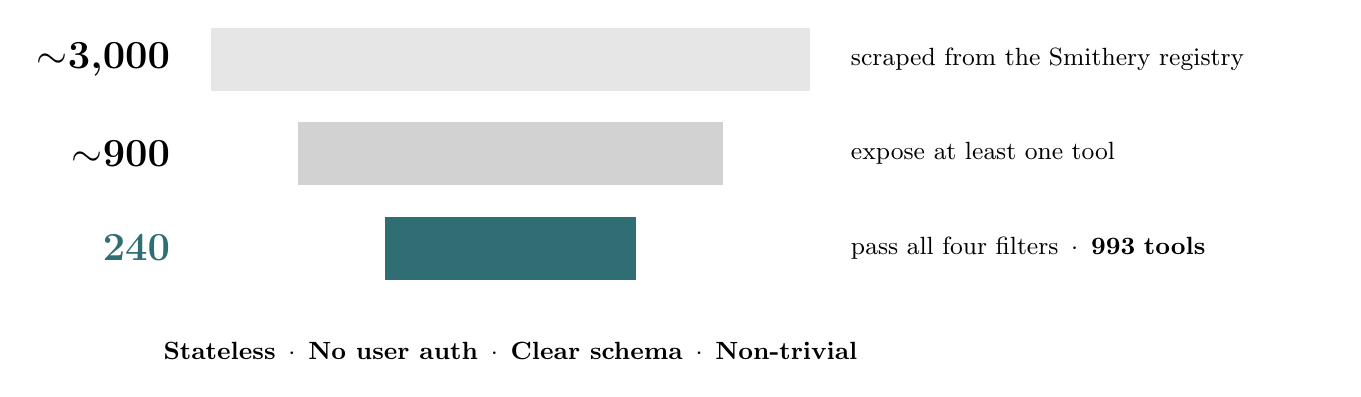
\begin{tikzpicture}[
      num/.style={font=\Large\bfseries, anchor=east},
      lab/.style={font=\small, anchor=west, text width=6cm, align=left}]
    \fill[barbase!25] (-3.8,2.0) rectangle (3.8,2.8);
    \fill[barbase!45] (-2.7,0.8) rectangle (2.7,1.6);
    \fill[barpos]     (-1.6,-0.4) rectangle (1.6,0.4);
    \node[num] at (-4.2,2.4) {$\sim$3,000};
    \node[lab] at (4.2,2.4) {scraped from the Smithery registry};
    \node[num] at (-4.2,1.2) {$\sim$900};
    \node[lab] at (4.2,1.2) {expose at least one tool};
    \node[num, barpos] at (-4.2,0) {240};
    \node[lab] at (4.2,0) {pass all four filters \,$\cdot$\, \textbf{993 tools}};
    \node[font=\small, align=center] at (0,-1.3)
      {\textbf{Stateless} \,$\cdot$\, \textbf{No user auth} \,$\cdot$\, \textbf{Clear schema} \,$\cdot$\, \textbf{Non-trivial}};
  \end{tikzpicture}}\\[8pt]
  {\small An LLM screens every server; a server must satisfy all four, spot-checked by hand.}
\end{frame}

\begin{frame}[t]{Tool Graph}
  \vspace{8pt}
  \centering
      \resizebox{!}{.66\textheight}{%
      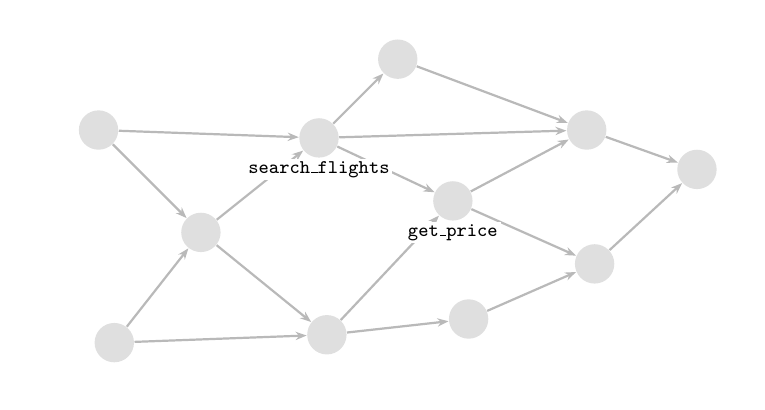
\begin{tikzpicture}[
          tn/.style={circle, fill=gray!25, minimum size=0.5cm, inner sep=0},
          ge/.style={-{Stealth[length=4pt]}, gray!55, line width=0.8pt}]
        \useasboundingbox (-2.2,-1.9) rectangle (6.8,2.6);
        \foreach \n/\x/\y in {a/0/0, b/1.5/1.2, c/1.6/-1.3, d/3.2/0.4, e/3.4/-1.1, f/4.9/1.3, g/5.0/-0.4, h/2.5/2.2, i/-1.3/1.3, j/-1.1/-1.4, k/6.3/0.8}
          \node[tn] (\n) at (\x,\y) {};
        \foreach \s/\t in {i/a, i/b, j/a, j/c, b/h, b/d, c/d, c/e, d/f, d/g, e/g, h/f, f/k, g/k, b/f, a/b, a/c}
          \draw[ge] (\s) -- (\t);
        \node[font=\scriptsize, anchor=north, fill=white, inner sep=1pt] at (b.south) {\ttfamily search\_flights};
        \node[font=\scriptsize, anchor=north, fill=white, inner sep=1pt] at (d.south) {\ttfamily get\_price};
      \end{tikzpicture}}\\[8pt]
  {\Large\textbf{993}}\,{\small tools} \quad
  {\Large\textbf{83K}}\,{\small edges: ``can $A$'s output feed $B$?''} \quad
  {\Large\textbf{88}}\,{\small successors per tool}
\end{frame}

\begin{frame}[t]{Graph-Guided Exploration}
  \vspace{8pt}
  \centering
      \resizebox{!}{.66\textheight}{%
      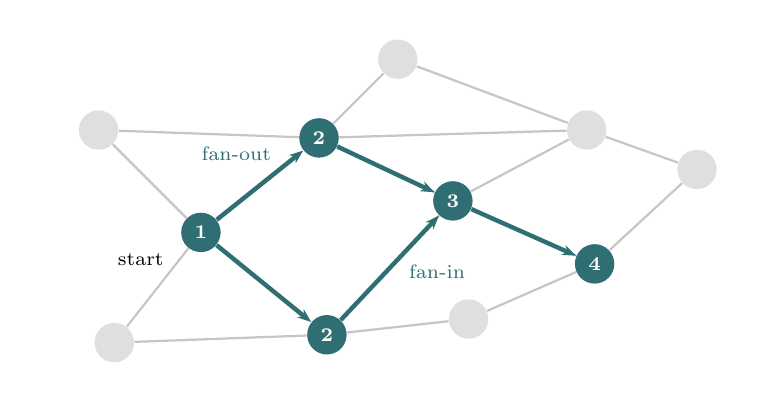
\begin{tikzpicture}[
          tn/.style={circle, fill=gray!25, minimum size=0.5cm, inner sep=0},
          hn/.style={circle, fill=barpos, text=white, minimum size=0.5cm, inner sep=0, font=\scriptsize\bfseries},
          ge/.style={gray!45, line width=0.8pt},
          he/.style={-{Stealth[length=5pt]}, barpos, line width=1.6pt}]
        \useasboundingbox (-2.2,-1.9) rectangle (6.8,2.6);
        \foreach \n/\x/\y in {a/0/0, b/1.5/1.2, c/1.6/-1.3, d/3.2/0.4, e/3.4/-1.1, f/4.9/1.3, g/5.0/-0.4, h/2.5/2.2, i/-1.3/1.3, j/-1.1/-1.4, k/6.3/0.8}
          \node[tn] (\n) at (\x,\y) {};
        \foreach \s/\t in {i/a, i/b, j/a, j/c, b/h, b/d, c/d, c/e, d/f, d/g, e/g, h/f, f/k, g/k, b/f}
          \draw[ge] (\s) -- (\t);
        \foreach \n/\l in {a/1, b/2, c/2, d/3, g/4}
          \node[hn] at (\n) {\l};
        \draw[he] (a) -- (b);
        \draw[he] (a) -- (c);
        \draw[he] (b) -- (d);
        \draw[he] (c) -- (d);
        \draw[he] (d) -- (g);
        \node[font=\scriptsize, anchor=east] at (-0.35,-0.35) {start};
        \node[font=\scriptsize\color{barpos}] at (0.45,1.0) {fan-out};
        \node[font=\scriptsize\color{barpos}] at (3.0,-0.5) {fan-in};
      \end{tikzpicture}}
\end{frame}

\begin{frame}{Back-Chaining: From Observed States to a Task}
  \centering
  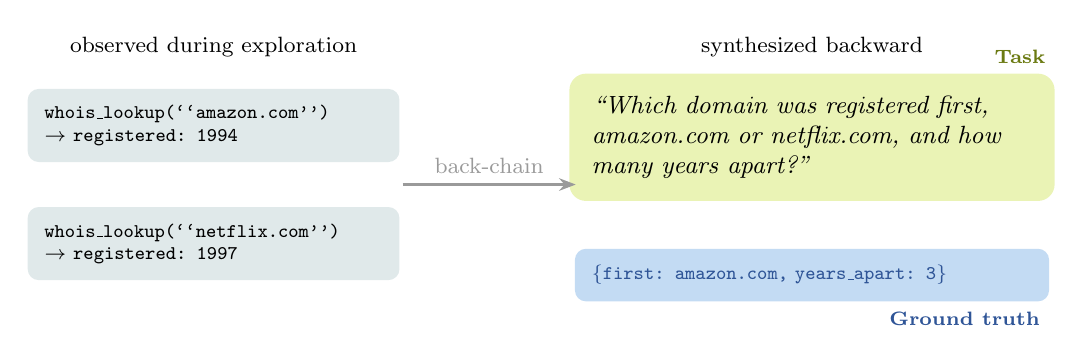
\begin{tikzpicture}[
      call/.style={fill=barpos!15, rounded corners=4pt, font=\ttfamily\scriptsize, align=left, inner sep=6pt, text width=4.3cm},
      arr/.style={-{Stealth[length=6pt]}, line width=1.2pt, tickgray}]
    \node[font=\footnotesize] at (0,1.9) {observed during exploration};
    \node[call] (c1) at (0,0.9) {whois\_lookup(``amazon.com'')\\$\rightarrow$ registered: 1994};
    \node[call] (c2) at (0,-0.6) {whois\_lookup(``netflix.com'')\\$\rightarrow$ registered: 1997};
    \node[font=\footnotesize] at (7.6,1.9) {synthesized backward};
    \node[fill=rsnbg, rounded corners=6pt, text width=5.6cm, align=left, inner sep=8pt, font=\small\itshape] (task) at (7.6,0.75)
      {``Which domain was registered first, amazon.com or netflix.com, and how many years apart?''};
    \node[fill=actbg, text=actfg, rounded corners=4pt, text width=5.6cm, align=left, inner sep=6pt, font=\ttfamily\scriptsize] (ans) at (7.6,-1.0)
      {\{first: amazon.com, years\_apart: 3\}};
    \node[rsnfg, font=\scriptsize\bfseries, anchor=south east] at (task.north east) {Task};
    \node[actfg, font=\scriptsize\bfseries, anchor=north east] at (ans.south east) {Ground truth};
    \draw[arr] (2.4,0.15) -- node[above, font=\footnotesize] {back-chain} (4.6,0.15);
  \end{tikzpicture}\\[12pt]
  {\small The task embeds the chosen nodes' inputs; the answer is read off their outputs.}\\
  {\small Unused nodes become distractors. Several tasks per DAG from different subsets.}
\end{frame}

\begin{frame}{Task Validation}
  \centering
  \resizebox{.96\linewidth}{!}{%
  \begin{tikzpicture}[
      card/.style={fill=gray!10, rounded corners=6pt, minimum width=2.5cm, minimum height=2.7cm},
      ico/.style={barpos, font=\fontsize{22}{22}\selectfont},
      nm/.style={font=\small\bfseries},
      ds/.style={font=\footnotesize, text width=2.3cm, align=center}]
    \foreach \x/\i/\n/\d in {
        0/\faCheckCircle/Verifiable/answer is objectively checkable,
        2.9/\faBullseye/Well-specified/exactly one correct answer,
        5.8/\faEye/Interpretable/no opaque IDs,
        8.7/\faGlobe/Realistic/realism $\geq$ 5 of 10,
        11.6/\faSignal/Calibrated/difficulty matches trajectory} {
      \node[card] at (\x,0) {};
      \node[ico] at (\x,0.75) {\i};
      \node[nm]  at (\x,0.0) {\n};
      \node[ds]  at (\x,-0.7) {\d};
    }
  \end{tikzpicture}}\\[14pt]
  {\Large\textbf{9,275}}\,{\small candidate tasks} \quad$\rightarrow$\quad {\Large\color{barpos}\textbf{5,144}}\,{\small pass all five, judged by an LLM}
\end{frame}

\begin{frame}{Why Not Train on Live Servers?}
  \centering
  \resizebox{.96\linewidth}{!}{%
  \begin{tikzpicture}[
      card/.style={rounded corners=8pt, minimum width=4.8cm, minimum height=4.6cm, fill=gray!10},
      ico/.style={barneg, font=\fontsize{26}{26}\selectfont},
      hd/.style={font=\large\bfseries},
      ex/.style={font=\small, text width=4.4cm, align=center, execute at begin node={\hyphenpenalty=10000}}]
    % 1. down
    \node[card] at (0,0) {};
    \node[ico] at (0,1.5) {\faPowerOff};
    \node[hd] at (0,0.6) {Servers go down};
    \node[ex] at (0,-0.85) {\texttt{search("hotels")}\\[4pt] $\rightarrow$ \texttt{503 Unavailable}};
    % 2. not reproducible
    \node[card] at (5.4,0) {};
    \node[ico] at (5.4,1.5) {\faCloudSun};
    \node[hd] at (5.4,0.6) {Not reproducible};
    \node[ex] at (5.4,-0.85) {\texttt{get\_weather("Boston")}\\[4pt] Mon $\rightarrow$ \texttt{18°C, sunny}\\ Tue $\rightarrow$ \texttt{9°C, rain}};
    % 3. random
    \node[card] at (10.8,0) {};
    \node[ico] at (10.8,1.5) {\faDice};
    \node[hd] at (10.8,0.6) {Random by design};
    \node[ex] at (10.8,-0.85) {\texttt{fortune\_telling("Leo")}\\[4pt] 1st $\rightarrow$ \texttt{"great luck"}\\ 2nd $\rightarrow$ \texttt{"beware Tuesday"}};
  \end{tikzpicture}}\\[14pt]
  {\small\bfseries The same call must return the same response, or the reward means nothing.}
\end{frame}

\begin{frame}{Replay Simulator: How It Works}
  \centering
  {\small Cached from exploration: \texttt{search(query="hotels", num=5, format="csv")}}\\[10pt]
  \resizebox{.96\linewidth}{!}{%
  \begin{tikzpicture}[
      card/.style={rounded corners=8pt, minimum width=4.8cm, minimum height=4.6cm},
      hd/.style={font=\large\bfseries},
      keys/.style={font=\small, minimum height=1.7cm},
      res/.style={font=\small, text width=4.6cm, align=center, anchor=north,
                  execute at begin node={\hyphenpenalty=10000}}]
    \newcommand{\ok}{{\color{barpos}\faCheck}}
    \newcommand{\no}{{\color{barneg}\faTimes}}
    % exact match
    \node[card, fill=barpos!15] at (0,0) {};
    \node[hd, barpos] at (0,1.8) {exact match};
    \node[keys] at (0,0.45) {\begin{tabular}{@{}l@{\hspace{14pt}}c@{}}
        \texttt{query="hotels"} & \ok \\[3pt] \texttt{num=5} & \ok \\[3pt] \texttt{format="csv"} & \ok \end{tabular}};
    \node[res] at (0,-0.75) {return the \textbf{real}\\ cached response};
    % fuzzy match
    \node[card, fill=rsnbg] at (5.4,0) {};
    \node[hd, rsnfg] at (5.4,1.8) {fuzzy match};
    \node[keys] at (5.4,0.45) {\begin{tabular}{@{}l@{\hspace{14pt}}c@{}}
        \texttt{query="hotels"} & \ok \\[3pt] \texttt{num=5} & \ok \\[3pt] \texttt{format="json"} & \no \end{tabular}};
    \node[res] at (5.4,-0.75) {an LLM \textbf{simulates} it:\\ the cached result as JSON};
    % no data
    \node[card, fill=barneg!15] at (10.8,0) {};
    \node[hd, barneg] at (10.8,1.8) {no data};
    \node[keys, text width=4.2cm, align=center] at (10.8,0.45) {tool never called\\ during exploration};
    \node[res] at (10.8,-0.75) {return an \textbf{error}};
  \end{tikzpicture}}\\[12pt]
  {\small\bfseries No live server is touched: the same call always gets the same response.}
\end{frame}

\begin{frame}{Why Replay Is Enough}
  \begin{columns}[c]
    \begin{column}{0.46\linewidth}
      \centering
      \resizebox{.95\linewidth}{!}{%
      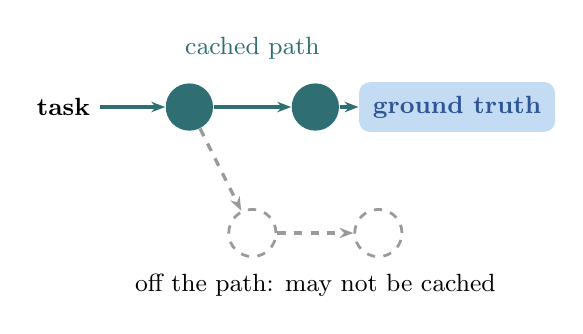
\begin{tikzpicture}[
          cn/.style={circle, fill=barpos, minimum size=0.6cm, inner sep=0},
          on/.style={circle, draw=barbase, dashed, line width=1pt, fill=white, minimum size=0.6cm, inner sep=0},
          he/.style={-{Stealth[length=5pt]}, barpos, line width=1.6pt},
          oe/.style={-{Stealth[length=5pt]}, barbase, dashed, line width=1.2pt}]
        \node[font=\small\bfseries] (s) at (0,0) {task};
        \node[cn] (c1) at (1.6,0) {};
        \node[cn] (c2) at (3.2,0) {};
        \node[fill=actbg, text=actfg, rounded corners=4pt, font=\small\bfseries, inner sep=5pt] (gt) at (5.0,0) {ground truth};
        \draw[he] (s) -- (c1);
        \draw[he] (c1) -- (c2);
        \draw[he] (c2) -- (gt);
        \node[font=\small, barpos] at (2.4,0.75) {cached path};
        \node[on] (o1) at (2.4,-1.6) {};
        \node[on] (o2) at (4.0,-1.6) {};
        \draw[oe] (c1) -- (o1);
        \draw[oe] (o1) -- (o2);
        \node[font=\small, anchor=north] at (3.2,-2.0) {off the path: may not be cached};
      \end{tikzpicture}}
    \end{column}
    \begin{column}{0.54\linewidth}
      {\small {\color{barpos}\faCheck}~\textbf{Correct agent}: stays on the path. Every call is cached, so it gets real responses and reaches the ground truth.}\\[10pt]
      {\small {\color{barneg}\faTimes}~\textbf{Wrong agent}: leaves the path and may hit missing data. That does not matter: it is already wrong, and its reward is 0 either way.}
    \end{column}
  \end{columns}
  \vspace{14pt}
  \centering
  {\small\bfseries Key assumption: every call on the path to the ground truth is cached.}\\
  {\small Back-chaining guarantees it: the task was written from those very calls.}
\end{frame}

\begin{frame}{RL Training}
  \centering
  \resizebox{.96\linewidth}{!}{%
  \begin{tikzpicture}[
      box/.style={rounded corners=6pt, minimum height=1.1cm, font=\small, align=center, inner sep=7pt},
      arr/.style={-{Stealth[length=6pt]}, line width=1.2pt, tickgray}]
    \node[box, fill=rsnbg] (task) at (0,0) {Task +\\tool schemas};
    \node[font=\fontsize{26}{26}\selectfont] (bot) at (3.0,0) {\faRobot};
    \node[font=\footnotesize, anchor=north] at (bot.south) {Qwen3-4B};
    \node[box, fill=barpos!15] (sim) at (6.4,0) {Replay\\simulator};
    \node[box, fill=actbg, text=actfg] (ans) at (9.6,0) {Final\\answer};
    \node[box, fill=gray!12] (rw) at (12.8,0) {Reward\\$\{0, 1\}$};
    \draw[arr] (task) -- (bot);
    \draw[arr] ([yshift=3pt]bot.east) -- node[above, font=\scriptsize, text=black] {tool call} ([yshift=3pt]sim.west);
    \draw[arr] ([yshift=-3pt]sim.west) -- node[below, font=\scriptsize, text=black] {response} ([yshift=-3pt]bot.east);
    \draw[arr] (sim) -- (ans);
    \draw[arr] (ans) -- (rw);
    \node[font=\footnotesize, align=center] at (12.8,-1.35) {exact field match,\\else LLM judge};
  \end{tikzpicture}}\\[18pt]
  {\small\bfseries GRPO with dynamic filtering}\\[10pt]
  {\Large\textbf{4,944}}\,{\small training tasks} \qquad {\Large\textbf{200}}\,{\small held-out test tasks}
\end{frame}

\section{Evaluation}

\begin{frame}{Evaluation Setup}
  \centering {\small\bfseries Does RL on \projectname help in distribution, and does it transfer?}
  \vspace{14pt}
  \begin{columns}[t]
    \begin{column}{0.32\linewidth}
      {\small\bfseries Model}\\[4pt]
      {\small Qwen3-4B-Thinking-2507, trained with RL on \projectname.}
    \end{column}
    \begin{column}{0.34\linewidth}
      {\small\bfseries Benchmarks}\\[4pt]
      {\small \projectname test set: 200 held-out tasks, pass@$k$ over 16 rollouts.}\\[4pt]
      {\small Tau2-Bench: Retail, Airline, Telecom.}\\[4pt]
      {\small MCP-Atlas and MCPMark.}
    \end{column}
    \begin{column}{0.32\linewidth}
      {\small\bfseries Baselines}\\[4pt]
      {\small The base checkpoint.}\\[4pt]
      {\small Claude Haiku 4.5, Sonnet 4.6, Opus 4.7 under the identical protocol.}
    \end{column}
  \end{columns}
\end{frame}

\begin{frame}{Results: A 4B Model Matches Claude Sonnet}
  \begin{columns}[c]
    \begin{column}{0.40\linewidth}
      \centering
      {\color{barpos}\fontsize{46}{50}\selectfont\textbf{41.5}}\\[2pt]
      {\small pass@1 on held-out \projectname tasks}\\
      {\small up from 28.1 before RL}\\[12pt]
      {\small Qwen3-4B after GRPO on \projectname\\ matches \textbf{Claude Sonnet 4.6} (42.2)}
    \end{column}
    \begin{column}{0.58\linewidth}
      \centering
      \resizebox{\linewidth}{!}{%
      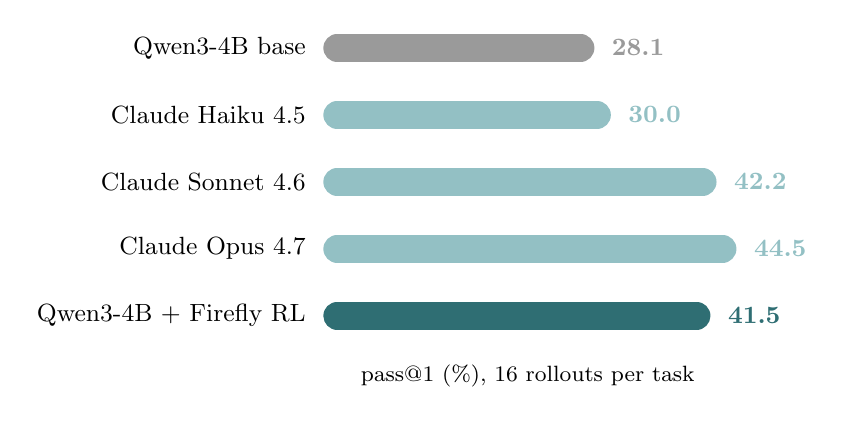
\begin{tikzpicture}[x=0.11cm,y=0.85cm]
        \foreach \y/\v/\c/\n in {4/28.1/barbase/Qwen3-4B base, 3/30.0/barsft/Claude Haiku 4.5, 2/42.2/barsft/Claude Sonnet 4.6, 1/44.5/barsft/Claude Opus 4.7, 0/41.5/barpos/Qwen3-4B + Firefly RL}{
          \draw[\c,line width=10pt,line cap=round] (0,\y) -- (\v,\y);
          \node[\c,anchor=west,font=\small\bfseries] at (\v+2.5,\y) {\v};
          \node[anchor=east,font=\small] at (-2.5,\y) {\n};
        }
        \node[font=\footnotesize] at (22,-0.9) {pass@1 (\%), 16 rollouts per task};
      \end{tikzpicture}}
    \end{column}
  \end{columns}
  \vspace{8pt}
  \centering {\small At pass@8 it reaches 52.8, above Sonnet (50.3) and close to Opus (54.4).}
\end{frame}

\begin{frame}{Results: It Transfers}
  \begin{table}[t]
    \centering
    \small
    \begin{booktabs}{
      colspec = {l X[c] X[c] X[c] X[c] X[c] X[c] X[c]},
      width = \linewidth,
      row{1,2} = {font=\bfseries},
      cell{1}{2} = {c=3}{c},
      cell{1}{5} = {c=1}{c},
      cell{1}{6} = {c=3}{c},
    }
    \toprule
    & Tau2-Bench & & & MCP-Atlas & MCPMark & & \\
    Model & Retail & Airline & Telecom & & File Sys. & PG Easy & PG Std \\
    \midrule
    Qwen3-4B              & 49.1 & 36.5 & 18.9 & 19.4 & 40.0 & 70.0 & 9.5 \\
    \textbf{+ \projectname RL} & \textbf{62.7} & \textbf{52.5} & \textbf{20.4} & \textbf{26.0} & \textbf{60.0} & \textbf{80.0} & \textbf{13.3} \\
    \bottomrule
    \end{booktabs}
  \end{table}
  \vspace{6pt}
  \centering {\small Improves on every public benchmark, \textbf{multi-turn} and \textbf{real MCP execution} included.}\\[2pt]
  {\small None of these tools or environments appear in \projectname.}
\end{frame}

\section{Conclusion}

\begin{frame}{Conclusion}
  \begin{columns}[c]
    \begin{column}{0.46\linewidth}
      \centering
      \resizebox{!}{.72\textheight}{\picktwotriangle{\node[fill=barpos, text=white, rounded corners=6pt, font=\bfseries, inner sep=7pt] at (0,-0.2) {\projectname};}}
    \end{column}
    \begin{column}{0.54\linewidth}
      {\small\textbf{Invert the pipeline.} Explore real APIs first, back-chain tasks from observed states: the ground truth is correct by construction.}\\[10pt]
      {\small\textbf{Scale it.} A tool graph steers exploration across 993 tools; a replay simulator removes drift from RL.}\\[10pt]
      {\small\textbf{It works.} 5,144 verified tasks take a 4B model to Claude Sonnet level, and the gains transfer.}
    \end{column}
  \end{columns}
\end{frame}

\begin{frame}[standout]
  \Large Thank you!

  Questions?

  \begin{tikzpicture}[remember picture,overlay]
    \node[anchor=south east] at ([xshift=-0.8cm,yshift=0.8cm]current page.south east) {
      \qrcode[height=2cm]{https://yuxuan.lu}
    };
  \end{tikzpicture}
\end{frame}

\end{document}
